%%%%%%%%%%%%%%%%%%%%%%%
% Section 
%%%%%%%%%%%%%%%%%%%%%%%
\section{Flexible Definition of 3D Systems}
\label{sect_flexibleDefinition}

Modia3D follows the approach of modern game engines to provide
a coordinate system as a primitive that is located in 3D and has a 
\textit{container with optional components} (such as geometry, visualization, dynamics, 
collision properties, light, camera, sound, etc.), see for example \cite{Nystrom2014}\footnote{\href{http://gameprogrammingpatterns.com/component.html}{http://gameprogrammingpatterns.com/component.html}}.\footnote{This section utilizes some descriptions, figures and Julia
code from \cite{Neumayr2018}.}
Such types of objects are called
\emph{GameObject}\footnote{\href{https://docs.unity3d.com/Manual/GameObjects.html}{https://docs.unity3d.com/Manual/GameObjects.html}} in Unity,
\emph{Actor}\footnote{\href{https://docs.unrealengine.com/en-us/Engine/Components}{https://docs.unrealengine.com/en-us/Engine/Components}} in Unreal Engine, and
\emph{Object3D}\footnote{\href{https://threejs.org/docs/index.html\#api/core/Object3D}{https://threejs.org/docs/index.html\#api/core/Object3D}} in Three.js. 
In Modia3D the name \emph{Object3D} is used. This very flexible approach allows to define many optional components and variants and treat them in a modular way. The Julia programming language is particularly suited for this \textit{component-oriented} programming pattern and therefore key-concepts of Julia, such as multiple dispatch, are heavily used in Modia3D. 
	
Hierarchical structuring for grouping and aggregation is performed with the Modia3D macro \texttt{@assembly}. Julia macros are metaprogramming\footnote{\href{https://docs.julialang.org/en/v1/manual/metaprogramming}{https://docs.julialang.org/en/v1/manual/metaprogramming}} language elements and a macro name starts with \texttt{@}. It generates an abstract syntax tree (AST) of Julia code which is automatically compiled and executed at the line where the macro is called. 
Fig.~\ref{fig:bar} shows a bar that is constructed from several Object3D elements
and is defined with the following Julia code:
\begin{lstlisting}[language = Julia]
@assembly Bar(;Lx=0.1,Ly=Lx/5,Lz=Ly) begin 
    obj0 = Object3D(Solid(SolidBeam(Lx,Ly,Lz), 
			"Aluminium", Material(color="Blue"))
	obj1 = Object3D(obj0,r=[-Lx/2,0.0,0.0]) 
	obj2 = Object3D(obj0,r=[ Lx/2,0.0,0.0]) 
end
\end{lstlisting}
\begin{figure}[htb]
	\centering
	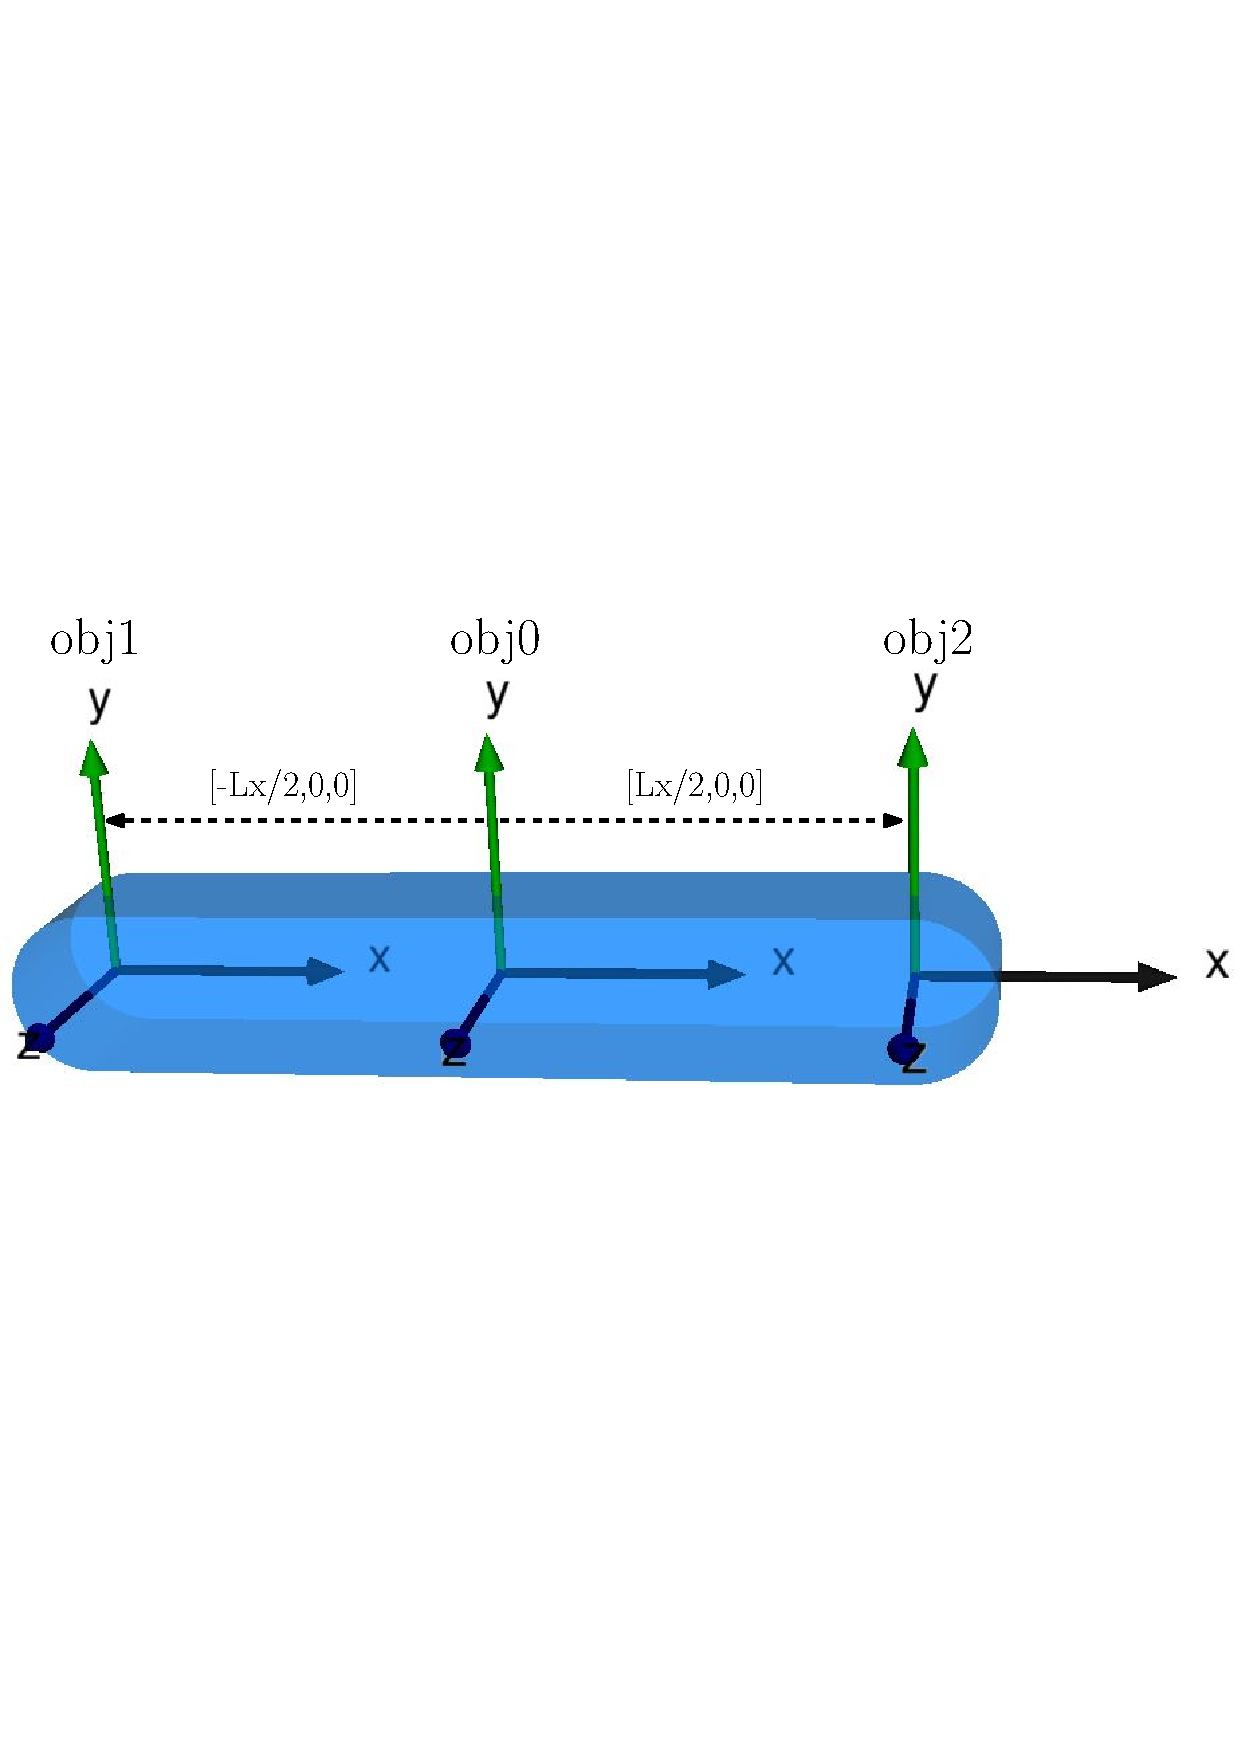
\includegraphics[width=0.3\textwidth]{figures/bar.pdf}  
	\caption{A solid bar with two additional Object3Ds.\label{fig:bar}}
\end{figure}
\begin{figure}[htb]
	\centering
	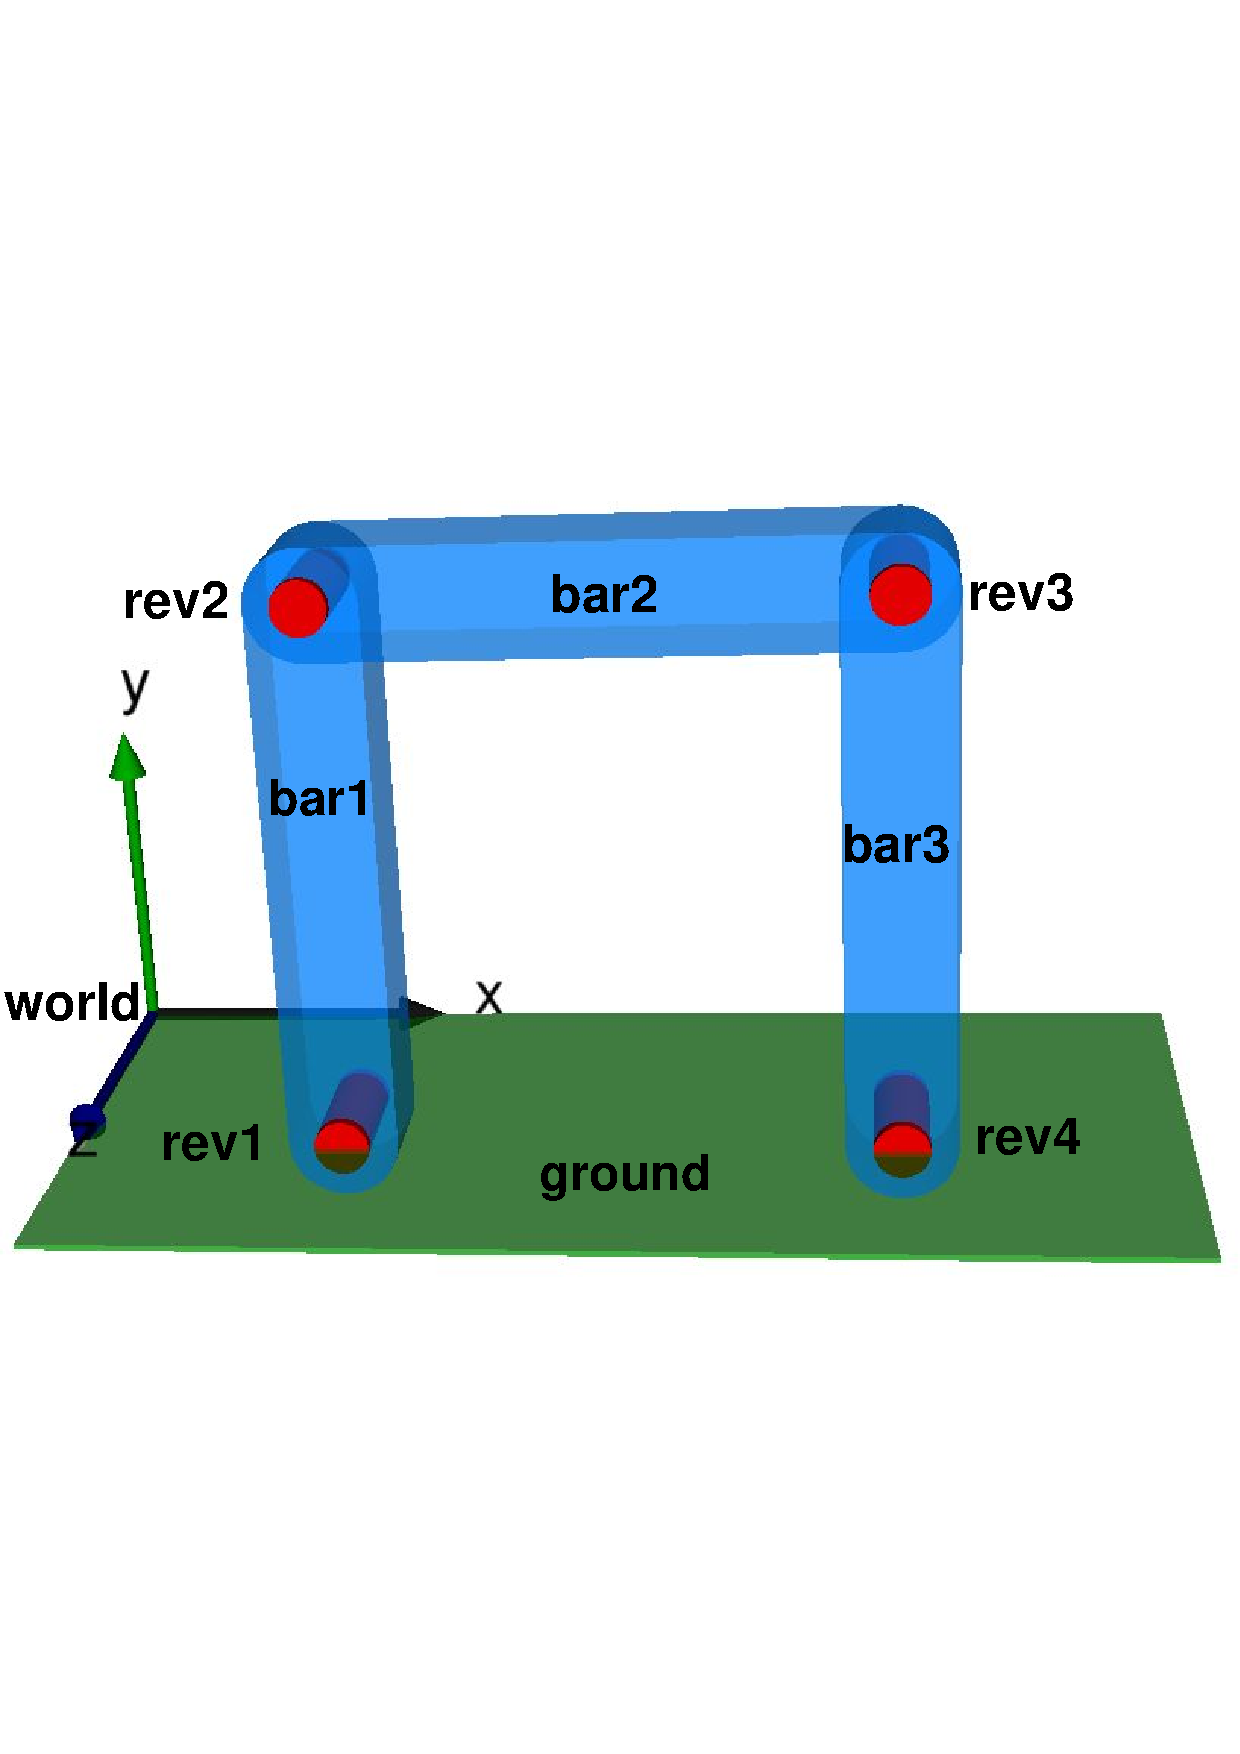
\includegraphics[width=0.3\textwidth]{figures/fourBar.pdf}  
	\caption{Planar four-bar mechanism.\label{fig:Fourbar}}
\end{figure}
The first Object3D is a \texttt{SolidBeam} geometry that is made of aluminium and is visualized in blue color. Mass, center of mass and inertia matrix are computed internally from this information. The next two objects place coordinate systems on the first object. Three instances of the \texttt{Bar} assembly together with a ground object  (= the fourth bar) are used to build up the four-bar mechanism\footnote{\href{https://en.wikipedia.org/wiki/Four-bar\_linkage}{https://en.wikipedia.org/wiki/Four-bar\_linkage}}
shown in Fig.~\ref{fig:Fourbar}.
The Julia code of this mechanism is shown in the next listing:
%
\begin{lstlisting}[language = Julia]
@assembly Fourbar(;Lx=0.1) begin
	world	= Object3D(CoordinateSystem(0.6)) 
	pos1 	= Object3D(world,r=[Lx/2,0.0,Lx/2]) 
	pos2 	= Object3D(pos1, r=[Lx,0.0,0.0]) 
	ground 	= Object3D(world,Box(..),..) 
	bar1	= Bar(Lx=Lx) 
	bar2	= Bar(Lx=Lx) 
	bar3	= Bar(Lx=Lx) 
	rev1	= Revolute(pos1,bar1.obj1,
				phi_start= pi/2) 
	rev2	= Revolute(bar1.obj2,bar2.obj1,				
				phi_start=-pi/2)	
	rev3	= Revolute(bar3.obj2,bar2.obj2, 			
				phi_start=-pi/2) 	
	rev4	= Revolute(pos2,bar3.obj1, 			
				phi_start= pi/2) 
	...
end
\end{lstlisting}
%
The angle of revolute joint \texttt{rev1} is moved kinematically via a signal. The resulting system
is simulated by calling function \texttt{simulate!} (for more details of 
the Modia3D elements, see \cite{Neumayr2018}):
% 
\begin{lstlisting}[language = Julia]
@assembly MoveFourBar(Lx=0.1) begin
	fourbar = Fourbar(Lx=Lx)
	sine 	= Sine(...)
	sig  	= SignalToFlangeAngle(sine.y)
	connect(sig, fourbar.rev1)
end

model  = SimulationModel(MoveFourBar(Lx=0.2))
result = simulate!(model, stopTime=3.0)
\end{lstlisting}
%
